%!TEX root = ../../Master.tex
\subsection{Formål}

Formålet med dette projekt er at udvikle et robotsystem. Der er fra kursets undervisere stillet krav om at system skal benytte sig af robotten AX-12A Smart Robotic Arm fra firmaet CrustCrawler Robotics. Desuden er der ligeledes stillet et krav om at systemet skal benytte sig af et vision system. \\

Det er valgt at udvikle et system til farvesortering af klodser. System skal ved hjælp af det anvendte vision system detekterer hvor klodserne befinder sig. Det skal herefter identificerer hvilke klodser der har samme farve og sorterer disse til hver sin side ved hjælp af robotten. Systemet skal blot kunne håndterer to forskellige farver. \\

\fixme{Ændre 'Figure' til 'Figur'}

\begin{figure}[h]
\centering
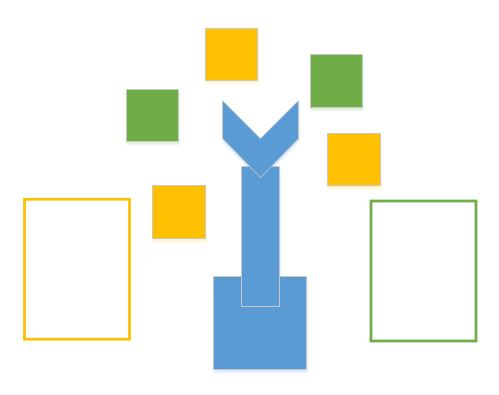
\includegraphics[scale=0.65]{images/purpose}
\caption{Idé til system setup}
\label{fig:purpose}
\end{figure}

En idé til system setup er illustreret i \autoref{fig:purpose}. Her ses robotten som den blå figur i midten. De grønne og gule kasser er de farvede klodser, som systemet skal kunne sortere. De markerede firkanter i siden er de steder, hvor klodserne skal placeres, når de er blevet sorteret. Disse markering forekommer kun på illustrationen og vil ikke være at finde i det endelige system.\\